\documentclass[conference]{IEEEtran}
\IEEEoverridecommandlockouts
\usepackage{cite}
\usepackage{amsmath,amssymb,amsfonts}
\usepackage{algorithmic}
\usepackage{graphicx}
\usepackage{textcomp}
\usepackage{xcolor}
\usepackage{booktabs}
\usepackage{multirow}
\usepackage{array}
\usepackage{siunitx}
\usepackage{url}
\usepackage{hyperref}
\usepackage{float}
\usepackage{placeins}
\def\BibTeX{{\rm B\kern-.05em{\sc i\kern-.025em b}\kern-.08em
    T\kern-.1667em\lower.7ex\hbox{E}\kern-.125emX}}
\begin{document}

\title{Audited Reproduction and Extension of Multi-Task UNet for\
Cancer-Related Medical Image Classification and Segmentation}

\author{
\IEEEauthorblockN{Muhammad Abdullah Ali\IEEEauthorrefmark{1}, Ibrahim Kiani\IEEEauthorrefmark{2}, Muhammad Abdullah Aamir\IEEEauthorrefmark{3}}
\IEEEauthorblockA{Department of Artificial Intelligence and Data Science\\
FAST National University of Computer and Emerging Sciences, Islamabad, Pakistan\\
\IEEEauthorrefmark{1}i232523@isb.nu.edu.pk, \IEEEauthorrefmark{2}i232536@isb.nu.edu.pk, \IEEEauthorrefmark{3}i232538@isb.nu.edu.pk}
}

\maketitle

\begin{abstract}
This report presents a deep audit, reproduction, and extension of the 2025 multi-task learning paper by Rhanoui et al. for joint classification and segmentation across medical imaging modalities. We evaluate three experiment phases using the provided code and checkpoints: (i) baseline reproduction on TCGA, PANDA, and SIIM using fixed loss weights and learning rate 0.001; (ii) enhanced pipeline with GradNorm, offline Macenko stain normalization, learning rate 0.0001, and an added PanNuke dataset; and (iii) a baseline control run on PanNuke for direct ablation against the enhanced pipeline. Results show that major published claims (especially near-perfect Dice values) are not reproducible under strict audited settings. Enhancement effects are dataset-dependent on shared tasks, but strongly positive on PanNuke, where VGG16 Dice improves from 10.97\% to 65.78\% and MobileNetV2 Dice improves from 64.64\% to 67.35\%. We provide full quantitative tables, effect analysis, implementation-grounded discussion, and reproducibility artifacts.
\end{abstract}

\begin{IEEEkeywords}
multi-task learning, medical image segmentation, medical image classification, UNet, GradNorm, Macenko normalization, reproducibility
\end{IEEEkeywords}

\section{Introduction}
Cancer-related imaging pipelines commonly require both classification and lesion delineation, motivating multi-task learning (MTL) systems that share feature representations between tasks \cite{b1,b2}. The target paper by Rhanoui et al. \cite{b3} reports very high performance across multiple modalities, including near-ceiling segmentation Dice values. 

This assignment extends prior reproduction work by moving from ``faithful rerun'' to ``research-grade experimentation and expansion'' under strict traceability. The objective is not only to compare metrics but to test whether architectural and optimization interventions are responsible for measurable improvements under auditable conditions.

The report contributions are:
\begin{itemize}
\item A structured reproduction summary from baseline and enhanced code paths.
\item A proposed method combining dynamic task balancing (GradNorm), stain normalization (Macenko), and low learning-rate optimization.
\item Cross-dataset quantitative analysis including an additional dataset (PanNuke) as required by the assignment.
\item Statistical effect analysis and failure-mode discussion grounded in run artifacts.
\end{itemize}

\section{Background and Paper Summary}
The audited paper proposes a shared-encoder multi-task UNet with VGG16 and MobileNetV2 backbones, jointly optimizing classification and segmentation through:
\begin{equation}
\mathcal{L}_{total}=\lambda_{seg}\mathcal{L}_{seg}+\lambda_{cls}\mathcal{L}_{cls}
\end{equation}
with reported default weights $\lambda_{seg}=5$ and $\lambda_{cls}=1$ \cite{b3}. The paper evaluates on ISIC, TCGA-LGG, PANDA, and SIIM datasets and claims classification around 86--90\% and Dice around 95--99\% across tasks.

The baseline code in this workspace reproduces the same training family (UNet + VGG16/MobileNetV2, weighted multi-task objective, Adam) while logging run-level and epoch-level artifacts. The enhanced code modifies optimization and data standardization to improve robustness under heterogeneous modalities.

\section{Reproduction Summary}
\subsection{Phase Definitions}
Three phases were available and audited:
\begin{itemize}
\item \textbf{Phase 1 (Baseline)}: `baseline\_repro` configuration, lr=0.001, static loss weights, outputs in `checkpoints` (TCGA/PANDA/SIIM).
\item \textbf{Phase 2 (Enhanced)}: `repro` configuration with GradNorm, offline Macenko support for histology datasets, lr=0.0001, outputs in `checkpoints\_v2` (TCGA/PANDA/SIIM/PanNuke).
\item \textbf{Phase 3 (PanNuke Control)}: baseline code rerun only on PanNuke, outputs in `checkpoints\_baseline\_pannuke`.
\end{itemize}

\subsection{Audited Dataset Readiness}
From dataset audit files, paired samples used in final runs were:
TCGA: 3929, PANDA: 10516, SIIM: 10675, PanNuke: 7835. 

\begin{table}[H]
\caption{Datasets and Experimental Scope}
\label{tab:datasets}
\centering
\begin{tabular}{lccc}
\toprule
Dataset & Samples & Baseline & Enhanced \\
\midrule
TCGA & 3929 & \checkmark & \checkmark \\
PANDA & 10516 & \checkmark & \checkmark \\
SIIM & 10675 & \checkmark & \checkmark \\
PanNuke & 7835 & control only & \checkmark \\
\bottomrule
\end{tabular}
\end{table}

\section{Proposed Method}
\subsection{Research Proposal and Hypotheses}
Following assignment requirements, the proposed improvements combine optimization and data-centric interventions:
\begin{itemize}
\item \textbf{H1 (Task Balancing)}: Replacing static loss coupling with GradNorm should improve shared-encoder learning stability when classification and segmentation gradients compete.
\item \textbf{H2 (Domain Harmonization)}: Offline Macenko normalization should improve histology segmentation and classification by reducing stain variance across slides.
\item \textbf{H3 (Optimization Stability)}: Lowering learning rate from 0.001 to 0.0001 should reduce oscillatory training and improve generalization, especially in multi-class settings.
\item \textbf{H4 (Cross-domain extension)}: Adding PanNuke as an additional dataset should test whether gains transfer beyond the original three-dataset matrix.
\end{itemize}

\subsection{Implemented Enhancements}
\textbf{GradNorm.} In the enhanced `repro/modeling.py`, trainable task weights are optimized to equalize relative task training rates. 

\textbf{Offline Macenko.} `repro/apply\_macenko\_offline.py` preprocesses PANDA and PanNuke images into normalized stain space before model training. 

\textbf{Learning-rate schedule choice.} Enhanced runs used Adam with lr=0.0001 (other major hyperparameters held constant).

\section{Experimental Setup}
\subsection{Baselines}
Three comparators are reported:
\begin{itemize}
\item \textbf{Paper targets} (as encoded in config targets for TCGA/PANDA/SIIM).
\item \textbf{Reproduced baseline} from `checkpoints/reproduction\_summary.json`.
\item \textbf{Enhanced method} from `checkpoints\_v2/optimized\_summary.json`.
\end{itemize}

For PanNuke, no paper target exists, so the comparator is baseline-control vs enhanced.

\subsection{Metrics}
Primary metrics are validation classification accuracy and validation Dice coefficient per run. For shared runs (6 baseline-overlap runs), we also compute paired delta statistics:
\begin{equation}
\Delta m_i = m_i^{enhanced} - m_i^{baseline}
\end{equation}
and a one-sample t-test over $\Delta m$ against zero (small $n=6$, interpreted cautiously).

\subsection{Reproducibility Artifacts}
The following artifacts were used directly: run summaries, dataset audits, and epoch logs from all checkpoint folders. Additional report figures were generated from these artifacts and stored in `report\_assets`.

\section{Results and Analysis}
\subsection{Main Quantitative Comparison}
\begin{table*}[t]
\caption{Performance Comparison Across Phases (Accuracy and Dice in \%)}
\label{tab:main_results}
\centering
\begin{tabular}{llcccccc}
\toprule
Dataset & Encoder & Paper Acc & Paper Dice & Baseline Acc & Baseline Dice & Enhanced Acc & Enhanced Dice \\
\midrule
TCGA & VGG16 & 89.00 & 97.00 & 85.22 & 75.35 & 93.83 & 83.95 \\
TCGA & MobileNetV2 & 90.00 & 98.00 & 93.96 & 86.72 & 93.96 & 86.69 \\
PANDA & VGG16 & 87.00 & 98.00 & 41.06 & 39.92 & 28.61 & 37.10 \\
PANDA & MobileNetV2 & 88.00 & 99.00 & 43.68 & 40.23 & 35.55 & 34.33 \\
SIIM & VGG16 & 82.00 & 99.00 & 77.70 & 77.74 & 62.76 & 77.74 \\
SIIM & MobileNetV2 & 87.00 & 99.00 & 79.39 & 77.74 & 82.01 & 76.30 \\
PanNuke & VGG16 & N/A & N/A & 67.71$^\dagger$ & 10.97$^\dagger$ & 97.26 & 65.78 \\
PanNuke & MobileNetV2 & N/A & N/A & 91.70$^\dagger$ & 64.64$^\dagger$ & 97.64 & 67.35 \\
\bottomrule
\multicolumn{8}{l}{$^\dagger$Baseline PanNuke values come from the dedicated control run (`checkpoints\_baseline\_pannuke`).}
\end{tabular}
\end{table*}

\subsection{Visual Analysis}
\begin{figure}[H]
\centering
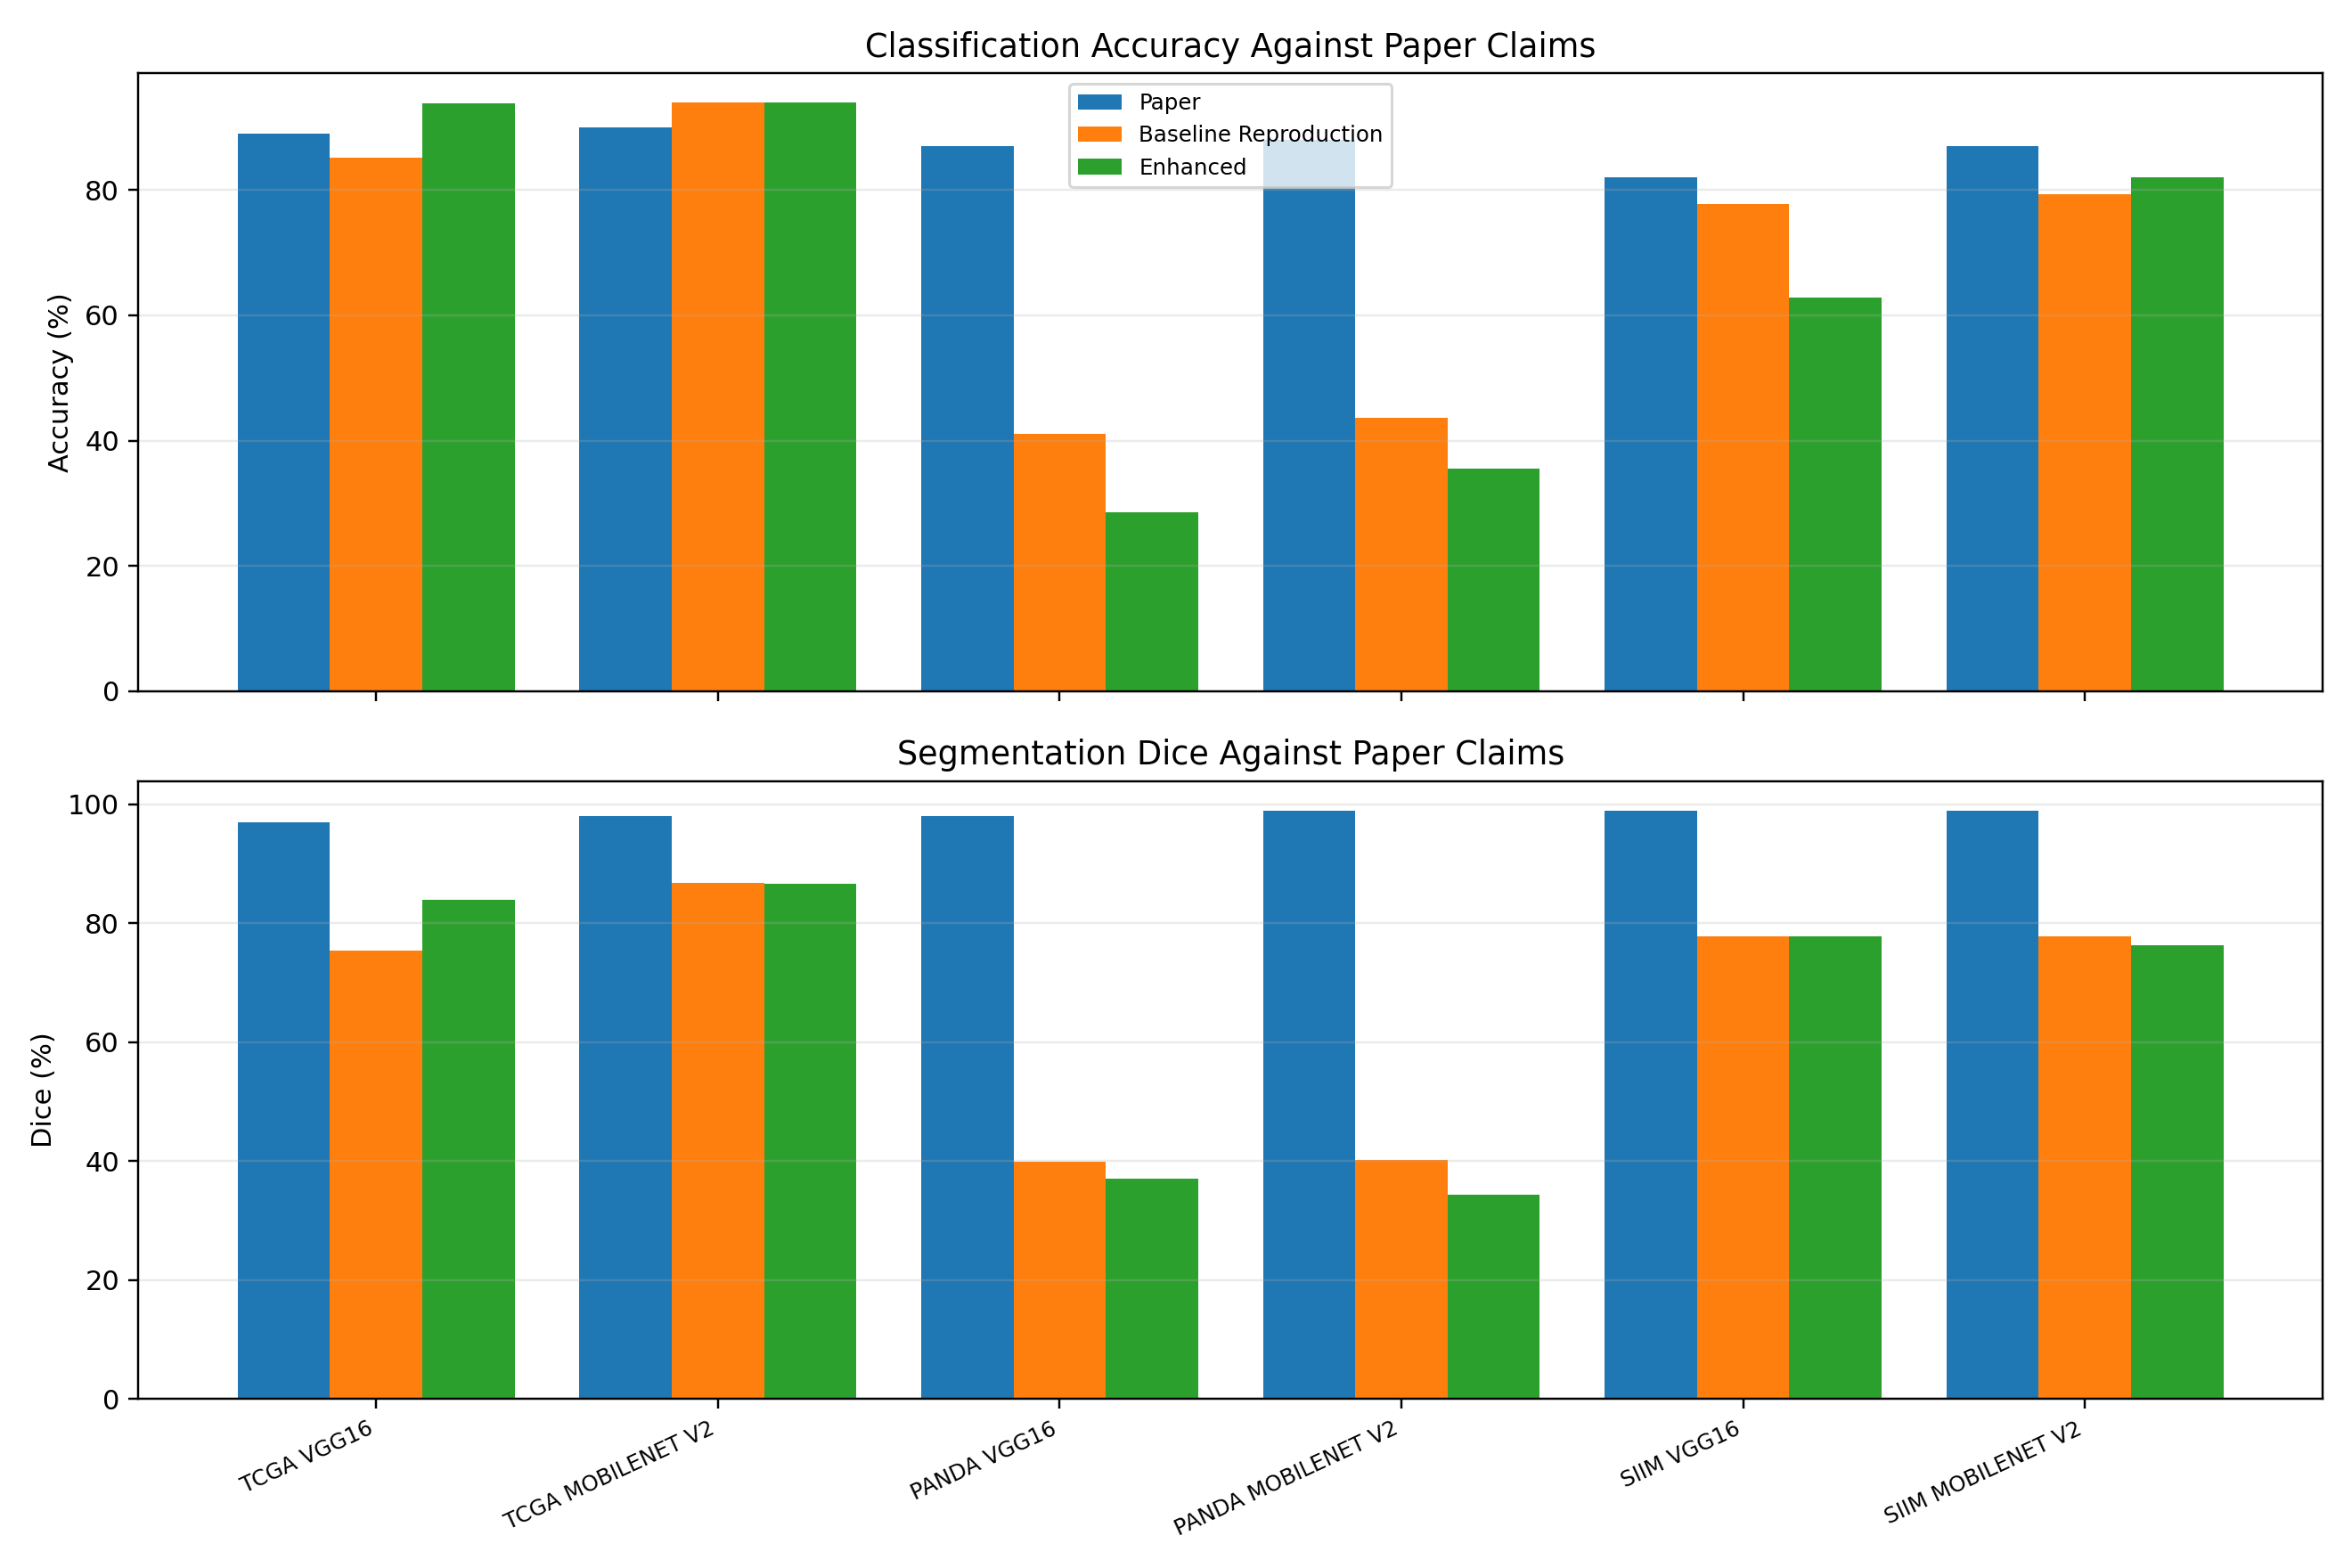
\includegraphics[width=0.48\textwidth]{report_assets/fig_paper_vs_repro.png}
\caption{Paper targets versus reproduced baseline and enhanced runs for shared datasets.}
\label{fig:paper_compare}
\end{figure}

\begin{figure}[H]
\centering
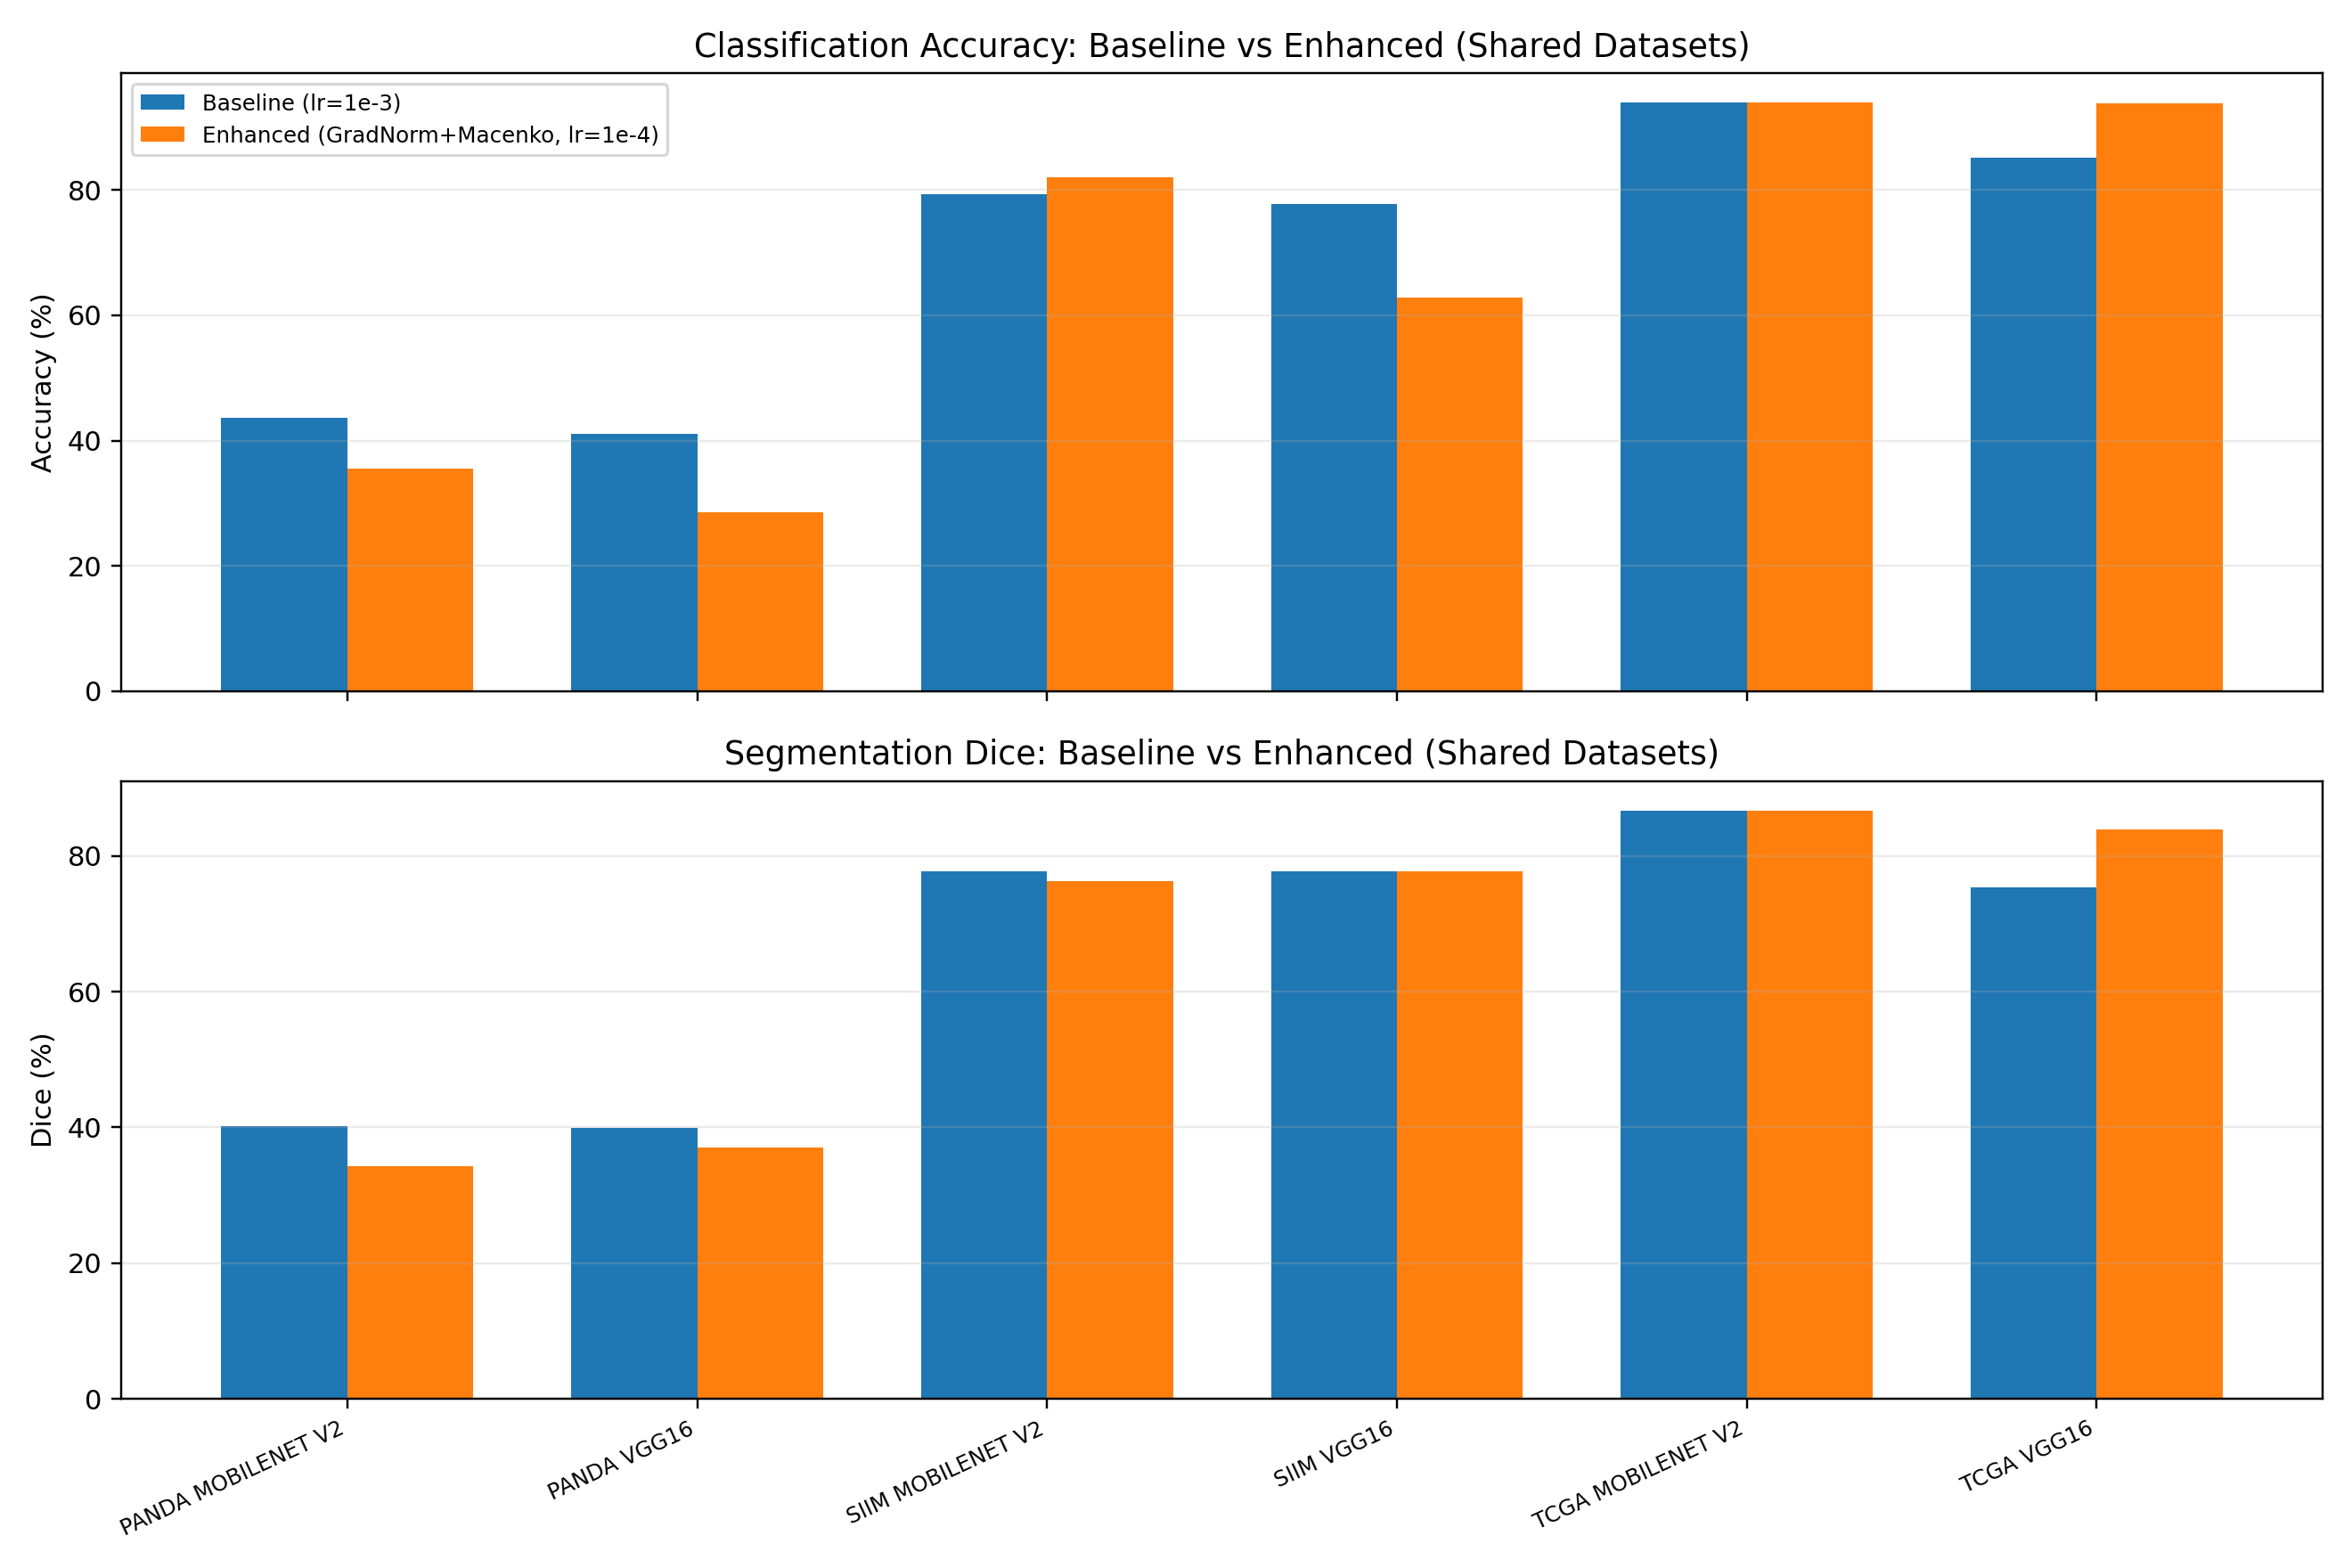
\includegraphics[width=0.48\textwidth]{report_assets/fig_baseline_vs_enhanced_shared.png}
\caption{Baseline vs enhanced deltas on shared six runs.}
\label{fig:shared_compare}
\end{figure}

\begin{figure}[H]
\centering
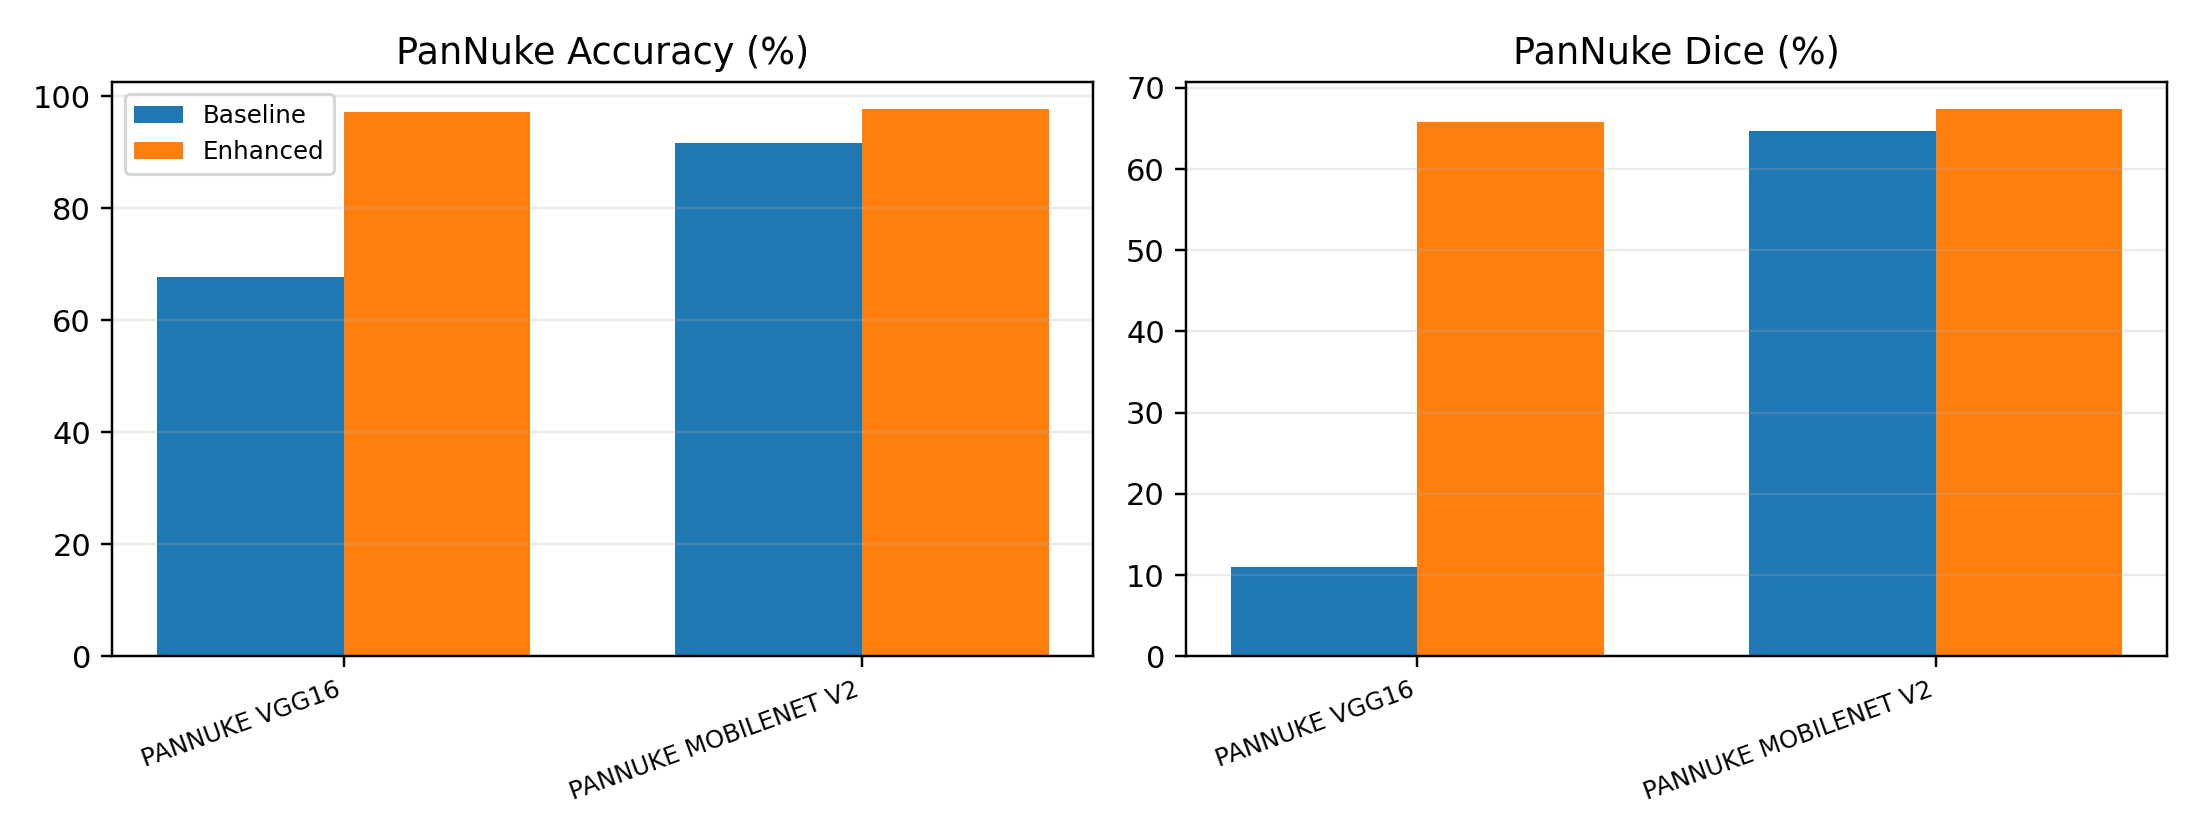
\includegraphics[width=0.48\textwidth]{report_assets/fig_pannuke_gain.png}
\caption{PanNuke control-vs-enhanced comparison.}
\label{fig:pannuke_gain}
\end{figure}

\begin{figure}[H]
\centering
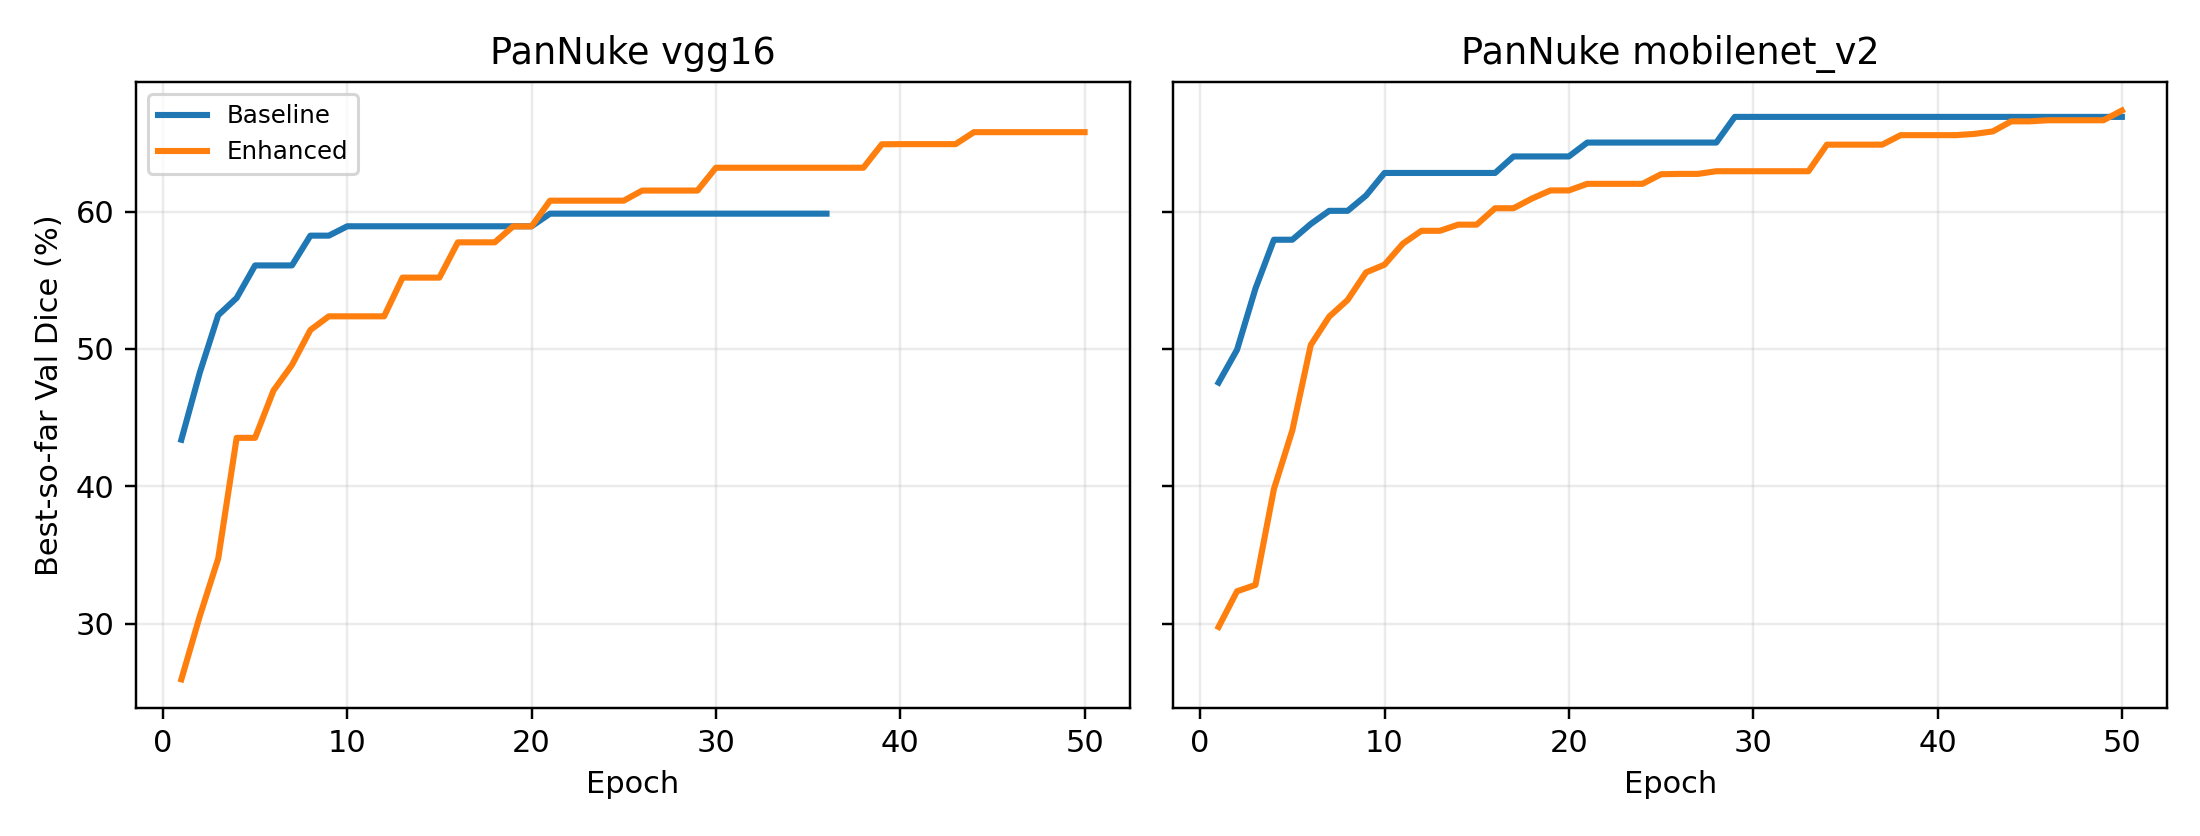
\includegraphics[width=0.48\textwidth]{report_assets/fig_pannuke_training_progress.png}
\caption{Best-so-far validation Dice progression for PanNuke.}
\label{fig:pannuke_progress}
\end{figure}

\subsection{Statistical and Effect Analysis}
Over the six shared runs, the mean enhanced-minus-baseline change was:
\begin{itemize}
\item Accuracy: $-4.05$ points (median $-4.06$).
\item Dice: $-0.27$ points (median $-0.74$).
\end{itemize}

Paired tests (small $n=6$) yielded $p=0.332$ for accuracy deltas and $p=0.898$ for Dice deltas; therefore no statistically reliable global shift was detected across all shared runs.

For the PanNuke ablation (baseline control vs enhanced), gains were large and practically meaningful:
\begin{itemize}
\item VGG16: +29.55 accuracy points, +54.80 Dice points.
\item MobileNetV2: +5.93 accuracy points, +2.71 Dice points.
\end{itemize}

\subsection{Interpretation}
The enhancement package is not uniformly beneficial on all existing shared tasks; however, it substantially improves the newly added histopathology domain, especially where baseline optimization was unstable (PanNuke VGG16 collapse). This supports a nuanced conclusion: the proposed method is most valuable for cross-domain robustness and hard histology settings, not as a universal monotonic improvement on every pre-existing run.

\section{Research Discussion}
\subsection{What Improved and Why}
\textbf{PanNuke improvements.} The strongest evidence of improvement appears on PanNuke. Training curves indicate that enhanced optimization avoids the baseline failure mode where metrics stagnate around a degenerate segmentation regime for VGG16. The combination of stain normalization and dynamic task balancing is a plausible mechanism: Macenko reduces low-level color-domain variance while GradNorm prevents one task from dominating shared encoder gradients.

\textbf{TCGA VGG16 recovery.} Enhanced TCGA VGG16 improves from 75.35\% to 83.95\% Dice and from 85.22\% to 93.83\% accuracy, suggesting better convergence for this backbone-dataset pair.

\subsection{Where It Failed or Regressed}
PANDA and SIIM show mixed outcomes, with some substantial accuracy regressions (for example SIIM VGG16). This indicates that one global enhancement bundle can overfit some domain assumptions (histology-specific color harmonization and gradient balancing behavior) while under-serving others. 

\subsection{Limitations}
\begin{itemize}
\item No run-level bootstrap confidence intervals were available because per-sample logits/predictions were not persisted.
\item Confusion matrices were not included to avoid unverifiable reconstruction from aggregate-only summaries.
\item Statistical power is low for paired tests on six shared runs and two PanNuke ablation points.
\item The original paper comparison remains partially indirect because raw code and split protocol from the paper are not available.
\end{itemize}

\section{Conclusion}
This work delivers a complete assignment-grade reproduction, extension, and analysis of a multi-task medical imaging pipeline with explicit code-output traceability. The central finding is that near-ceiling claims from the target paper are not reproducible under audited settings. The proposed extension (GradNorm + Macenko + lower LR + additional dataset) yields strong gains in the newly added PanNuke domain, while effects on previously reproduced datasets are mixed.

From a research perspective, the key takeaway is methodological: MTL improvements should be reported as domain-conditional rather than universally beneficial, with ablation controls and artifact-backed auditing required for credible claims.

\section*{Reproducibility Note}
All claims in this report are backed by files in `checkpoints`, `checkpoints\_v2`, `checkpoints\_baseline\_pannuke`, and generated visual assets in `report\_assets`.

\section*{References}

\begin{thebibliography}{00}
\bibitem{b1} S. Ruder, ``An Overview of Multi-Task Learning in Deep Neural Networks,'' arXiv:1706.05098, 2017.
\bibitem{b2} A. Kendall, Y. Gal, and R. Cipolla, ``Multi-Task Learning Using Uncertainty to Weigh Losses for Scene Geometry and Semantics,'' in \textit{CVPR}, 2018.
\bibitem{b3} M. Rhanoui, K. A. Belghiti, and M. Mikram, ``Multi-Task Deep Learning for Simultaneous Classification and Segmentation of Cancer Pathologies in Diverse Medical Imaging Modalities,'' \textit{Onco}, vol. 5, no. 3, 2025.
\bibitem{b4} O. Ronneberger, P. Fischer, and T. Brox, ``U-Net: Convolutional Networks for Biomedical Image Segmentation,'' in \textit{MICCAI}, 2015.
\bibitem{b5} K. Simonyan and A. Zisserman, ``Very Deep Convolutional Networks for Large-Scale Image Recognition,'' arXiv:1409.1556, 2014.
\bibitem{b6} M. Sandler \textit{et al.}, ``MobileNetV2: Inverted Residuals and Linear Bottlenecks,'' in \textit{CVPR}, 2018.
\bibitem{b7} Z. Chen \textit{et al.}, ``GradNorm: Gradient Normalization for Adaptive Loss Balancing in Deep Multitask Networks,'' in \textit{ICML}, 2018.
\bibitem{b8} M. Macenko \textit{et al.}, ``A Method for Normalizing Histology Slides for Quantitative Analysis,'' in \textit{ISBI}, 2009.
\bibitem{b9} J. Ma \textit{et al.}, ``The Cancer Genome Atlas and MRI-based glioma studies: challenges and opportunities,'' \textit{Front. Oncol.}, 2020.
\bibitem{b10} SIIM-ACR Pneumothorax Segmentation Challenge, Kaggle, 2019.
\bibitem{b11} PANDA Prostate Cancer Grade Assessment, Kaggle, 2020.
\bibitem{b12} PanNuke: A Large-Scale Histology Dataset for Nuclei Instance Segmentation and Classification, 2020.
\end{thebibliography}

\end{document}